\documentclass[journal,12pt,twocolumn]{IEEEtran}

\usepackage{setspace}
\usepackage{gensymb}
\singlespacing
\usepackage[cmex10]{amsmath}

\usepackage{amsthm}
\usepackage{commath}
\usepackage{mathrsfs}
\usepackage{txfonts}
\usepackage{stfloats}
\usepackage{bm}
\usepackage{cite}
\usepackage{cases}
\usepackage{subfig}

\usepackage{longtable}
\usepackage{multirow}

\usepackage{enumitem}
\usepackage{mathtools}
\usepackage{steinmetz}
\usepackage{tikz}
\usepackage{circuitikz}
\usepackage{verbatim}
\usepackage{tfrupee}
\usepackage[breaklinks=true]{hyperref}
\usepackage{graphicx}
\usepackage{tkz-euclide}

\usetikzlibrary{calc,math}
\usepackage{listings}
    \usepackage{color}                                            %%
    \usepackage{array}                                            %%
    \usepackage{longtable}                                        %%
    \usepackage{calc}                                             %%
    \usepackage{multirow}                                         %%
    \usepackage{hhline}                                           %%
    \usepackage{ifthen}                                           %%
    \usepackage{lscape}     
\usepackage{multicol}
\usepackage{chngcntr}

\DeclareMathOperator*{\Res}{Res}

\renewcommand\thesection{\arabic{section}}
\renewcommand\thesubsection{\thesection.\arabic{subsection}}
\renewcommand\thesubsubsection{\thesubsection.\arabic{subsubsection}}

\renewcommand\thesectiondis{\arabic{section}}
\renewcommand\thesubsectiondis{\thesectiondis.\arabic{subsection}}
\renewcommand\thesubsubsectiondis{\thesubsectiondis.\arabic{subsubsection}}
\newtheorem{theorem}{Theorem}[section]
\newtheorem{corollary}{Corollary}[theorem]
\newtheorem{lemma}[theorem]{Lemma}
\newtheorem{definition}{Definition}[section]

\hyphenation{op-tical net-works semi-conduc-tor}
\def\inputGnumericTable{}                                 %%

\lstset{
%language=C,
frame=single, 
breaklines=true,
columns=fullflexible
}
\begin{document}

\newcommand{\BEQA}{\begin{eqnarray}}
\newcommand{\EEQA}{\end{eqnarray}}
\newcommand{\define}{\stackrel{\triangle}{=}}
\bibliographystyle{IEEEtran}
\raggedbottom
\setlength{\parindent}{0pt}
\providecommand{\mbf}{\mathbf}
\providecommand{\pr}[1]{\ensuremath{\Pr\left(#1\right)}}
\providecommand{\qfunc}[1]{\ensuremath{Q\left(#1\right)}}
\providecommand{\sbrak}[1]{\ensuremath{{}\left[#1\right]}}
\providecommand{\lsbrak}[1]{\ensuremath{{}\left[#1\right.}}
\providecommand{\rsbrak}[1]{\ensuremath{{}\left.#1\right]}}
\providecommand{\brak}[1]{\ensuremath{\left(#1\right)}}
\providecommand{\lbrak}[1]{\ensuremath{\left(#1\right.}}
\providecommand{\rbrak}[1]{\ensuremath{\left.#1\right)}}
\providecommand{\cbrak}[1]{\ensuremath{\left\{#1\right\}}}
\providecommand{\lcbrak}[1]{\ensuremath{\left\{#1\right.}}
\providecommand{\rcbrak}[1]{\ensuremath{\left.#1\right\}}}
\theoremstyle{remark}
\newtheorem{rem}{Remark}
\newcommand{\sgn}{\mathop{\mathrm{sgn}}}
\providecommand{\abs}[1]{\vert#1\vert}
\providecommand{\res}[1]{\Res\displaylimits_{#1}} 
\providecommand{\norm}[1]{\lVert#1\rVert}
%\providecommand{\norm}[1]{\lVert#1\rVert}
\providecommand{\mtx}[1]{\mathbf{#1}}
\providecommand{\mean}[1]{E[ #1 ]}
\providecommand{\fourier}{\overset{\mathcal{F}}{ \rightleftharpoons}}
%\providecommand{\hilbert}{\overset{\mathcal{H}}{ \rightleftharpoons}}
\providecommand{\system}{\overset{\mathcal{H}}{ \longleftrightarrow}}
	%\newcommand{\solution}[2]{\textbf{Solution:}{#1}}
\newcommand{\solution}{\noindent \textbf{Solution: }}
\newcommand{\cosec}{\,\text{cosec}\,}
\providecommand{\dec}[2]{\ensuremath{\overset{#1}{\underset{#2}{\gtrless}}}}
\newcommand{\myvec}[1]{\ensuremath{\begin{pmatrix}#1\end{pmatrix}}}
\newcommand{\mydet}[1]{\ensuremath{\begin{vmatrix}#1\end{vmatrix}}}

\numberwithin{equation}{subsection}
\makeatletter
\@addtoreset{figure}{problem}
\makeatother
\let\StandardTheFigure\thefigure
\let\vec\mathbf
\renewcommand{\thefigure}{\theproblem}
\def\putbox#1#2#3{\makebox[0in][l]{\makebox[#1][l]{}\raisebox{\baselineskip}[0in][0in]{\raisebox{#2}[0in][0in]{#3}}}}
     \def\rightbox#1{\makebox[0in][r]{#1}}
     \def\centbox#1{\makebox[0in]{#1}}
     \def\topbox#1{\raisebox{-\baselineskip}[0in][0in]{#1}}
     \def\midbox#1{\raisebox{-0.5\baselineskip}[0in][0in]{#1}}
\vspace{3cm}
\title{Quiz 1}
\author{Savarana Datta - AI20BTECH11008}
\maketitle
\newpage
\bigskip
\renewcommand{\thefigure}{\theenumi}
\renewcommand{\thetable}{\theenumi}
Download latex-tikz codes from 
%
\begin{lstlisting}
https://github.com/SavaranaDatta/EE3900/blob/main/EE3900_Quiz1
\end{lstlisting}
\section{Question}
For the following signal determine whether the system is (1) stable, (2) casual, (3) linear and (4) time invariant.
\begin{align}
    T(x[n])=x[n^{2}]
\end{align}
\section{Solution}
\begin{figure}[htp]
    \centering
    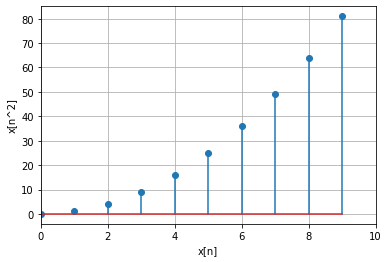
\includegraphics[width=\columnwidth]{fig.png}
    \caption{plot of the system}
\end{figure}
\begin{definition}{\textbf{Stable}}
A system is said to be BIBO stable if the response to a bounded input is always bounded.
\end{definition} 

As the given signal input $x[n]$ is bounded,
\begin{align}
   |x[n]| < M \text{   for some real $M$}\\
   \text{Hence  } |x[n^{2}]| < M
\end{align}
So $x[n^{2}]$ is also bounded. Hence, the system is stable i.e, bounded input bounded output stable.\\

\begin{definition}{\textbf{Casual}}
 The output at any instant does not depend on the future inputs i.e, for at $n_{0}$ y[$n_{0}$] does not depend on x[n] for $n>n_{0}$.
\end{definition}

Here, for this signal the output depends on x[$n_{0}^{2}$]. As $n_{0}$ is an integer $n_{0}^{2}>n_{0}$ for $n_{0}>1$ .\\
For example consider n=2
\begin{align}
    x[2] \implies x[4]
\end{align}
Here the output for n=2 depends on n=4. So the output depends on the future input. Hence, the system is non casual.

\begin{definition}{\textbf{Linear}}
The response to an arbitary linear combination of input signals is always the same linear combinations of the individual responses to these signals 
\end{definition}
\begin{align}
    x_{1}[n] \implies x_{1}[n^{2}]\\
    x_{2}[n] \implies x_{2}[n^{2}]
\end{align}
\begin{align}
    ax_{1}[n]+bx_{2}[n] \implies ax_{1}[n^{2}]+bx_{2}[n^{2}]
\end{align}
As this system obeys both law of addition and law of homogenity, the given system is linear.

\begin{definition}{\textbf{Time Invariant}}
The response to an arbitrary translated set of inputs is always the response to the original set, but translated by the same amount.\\
If 
\begin{align}
    x[n]\implies y[n]
\end{align}
then
\begin{align}
    x[n-n_{0}] \implies y[n-n_{0}]
\end{align} for all x and $n_{0}$.
\end{definition}
Here 
\begin{align}
    x[n]\implies x[n^{2}]
\end{align}
adding time delay($n_{0}$) to the output signal
\begin{align}
\label{eq1}
    x[n^{2}]\implies x[(n-n_{0})^{2}]
\end{align}
adding time delay($n_{0}$) to the input signal 
\begin{align}
    x[n]\implies x[n-n_{0}]
\end{align}
Now the ouput signal 
\begin{align}
\label{eq2}
    x[n-n_{0}]\implies x[n^{2}-n_{0}]
\end{align}
As \ref{eq1} and \ref{eq2} are not same, the given signal is time variant. 
\end{document}


